
\documentclass[a4paper,12pt, oneside]{book}

%  Русский язык
\usepackage{cmap}					% Улучшенный поиск русских слов
\usepackage[T2A]{fontenc}			% кодировка
\usepackage[utf8]{inputenc}			% кодировка исходного текста
\usepackage[english,russian]{babel}	% локализация и переносы
\usepackage{pscyr}					% нормальные шрифты

% Колонтитулы
\usepackage{fancybox,fancyhdr}
\usepackage{lastpage}
\fancyhf{}
\fancypagestyle{all}
{
	\fancyhead{}
	\fancyhead[C]{\vspace{-5mm}Контрольная работа 12 Вариант Попов Юрий СКБ-171\vspace{3mm}}
	\fancyfoot{}
	\fancyfoot[C]{\hfill  \thepage  \hfill}
}

% Картинки и графики
\usepackage{wrapfig}
\usepackage{pgfplots}
\pgfplotsset{compat=1.9}

% Ссылки
\usepackage{xcolor}
\usepackage{color,colortbl} % раскраска таблиц
\usepackage[unicode, pdftex]{hyperref}
\definecolor{linkcolor}{HTML}{000000} 	% цвет ссылок
\definecolor{urlcolor}{HTML}{8B000F}	% цвет гиперссылок
\hypersetup{urlcolor=urlcolor, linkcolor=linkcolor, colorlinks=true}

% Размеры
\setlength{\paperwidth}{210mm}
\setlength{\paperheight}{297mm}
\setlength{\textheight}{225mm} 			% высота без колонтитулов
\setlength{\textwidth}{170mm}			% ширина текста
\oddsidemargin=0pt
\setlength{\headheight}{2mm}			% высота колонтитула
\setlength{\headsep}{5mm} 	% от блока текста до верхнего колонтитула
\setlength{\footskip}{10mm}  % от блока текста до нижнего колонтитула

% Математика
\usepackage{amsmath,amsfonts,amssymb,amsthm,mathtools,mathtext} 
\usepackage{latexsym,array,epsfig,wasysym}
\usepackage[all]{xy}
\let\int\varint
\def\Int{\int\limits}
\def\IInt{\iint\limits}
\def\IIInt{\iiint\limits}
\DeclarePairedDelimiter\floor{\lfloor}{\rfloor}


% Оглавление 
\usepackage{setspace}

\usepackage{tocloft} %регулировка расположения TableOfContent (Оглавления) на странице

%\setcounter{tocdepth}{1} % отменяет вывод в оглавление subsection and subsubsection
%\setcounter{secnumdepth}{1} %отменяет номерацию секций в тексте и оглавлении.
\usepackage{tocloft} %регулировка расположения TableOfContent (Оглавления) на странице

\renewcommand{\cfttoctitlefont}{\hspace{0.38\textwidth} \bfseries\MakeUppercase} %уменьшаем размер шрифта и ровняем по центру

% % Межстрочные отступы в Оглавлении:
\setlength{\cftbeforetoctitleskip}{5mm} %отступ Оглавления от верхнего поля страницы.
\setlength{\cftbeforechapskip}{14mm} %отступ между главами
\setlength{\cftbeforesecskip}{5mm} %отступ между секциями \section{title}

% % Отступы от левого поля:
\setlength{\cftchapindent}{1mm} %отступ между левым полем и \chapter{}
\setlength{\cftsecindent}{13mm} %отступ между левым полем и \section{title}

% % Отточия в Оглавлении
\renewcommand\cftchapdotsep{\cftdot} %добавляет отточия после \chapter{title}
%\renewcommand{\cftchapleader}{\cftdotfill{\cftchapdotsep}} %делает отточия после \chapter{title} тонкими, (по умолчанию жирные).
\renewcommand\cftsecdotsep{\cftdot} %делает отточия после \section{title} частыми.

% % Интервалы между абзацами, главами и так далее:
\usepackage{titlesec}

\titleformat{\chapter}[display]
{\filcenter}
{\MakeUppercase{\chaptertitlename} \thechapter}
{8pt}
{\bfseries}{}

\titleformat{\section}
{\normalsize\bfseries}
{\thesection}
{1em}{}

\titleformat{\subsection}
{\normalsize\bfseries}
{\thesubsection}
{1em}{}

% Настройка вертикальных и горизонтальных отступов
\titlespacing*{\chapter}{0pt}{-30pt}{8pt}
\titlespacing*{\section}{\parindent}{*4}{*4}
\titlespacing*{\subsection}{\parindent}{*4}{*4}


\begin{document} % начало документа	
	\pagestyle{plain}
	
	\begin{titlepage}	
		\begin{center}
			{\Huge \textbf{Математическая статистика}}
			\vspace{30mm}
			
			{\Huge Домашняя работа № 2 \\}
			\vspace{30mm}
			
			{\huge Основные понятия 
				
				математической статистики}
			\vspace{30mm}
			
			{\Large Попов Юрий, СКБ-172}
		\end{center}
	\end{titlepage}
	
	
	
	\begin{spacing}{0.99}          
		\tableofcontents %Оглавление. Корректно создается за два прогона tex файла.               
	\end{spacing}

\newpage
\begin{center}
	{\Huge{\bf{Предисловие}}}
\end{center}

%-------------------------------------Предисловие
\vspace{5mm}
Все графики, которые в дальнейшем будут вставлены в эту работу, были сконструированы с помощью различных библиотек, основные которые - это matplotlib  и numpy в Jupyter Notebook

К работе приложены 2 основных файла: DZ\_2\_Geom и DZ\_2\_Exp, в которых указаны расчеты  соотвественно геометрического и  экспоненциального распределения

Также есть файл get\_quantile\_geom, в котором расписан процесс нахождения квантиля.
\vspace{5mm}

Большая часть определений, которые представлены в этой работы взять с лекций нашего курса. 
\vspace{5mm}

Также некоторые определения взяты из источника   Г.И. Ивченко, Ю.И. Медведев \\
"Ведение в математическую статистику"

\setcounter{secnumdepth}{-1} % убираем нумерацию 
%-------------------------------------Предисловие
 
\newpage
{\large\textit{\textbf{Задание 2.1} Моделирование выбранных случайных величин}}
\addcontentsline{toc}{chapter}{Задание 2.1 Моделирование выбранных случайных величин}

\vspace{5mm}
	\large{\textbf{Реализация выборки}}
\vspace{5mm}

\normalsize{\textbf{Определение 1.}} \textit{Реализация выборки - }это набор из n наблюдений $\hat{x} = (x_1, x_2, \ldots, x_n)$

\vspace{5mm}
\text{\large{\textbf {2.1.1 Геометрическое распределение}}}\\
\addcontentsline{toc}{section}{2.1.1 Геометрическое распределение}
\vspace{5mm}

Используя итоговый из задания 1 для моделирования случайных величин, подчиняющих геометрическому распределению, были построены по 5 реализаций выборок различных объемов(5, 10, 100, 1000, 10**5)
\vspace{5mm}

Вот, пример по  5 реализаций выборки объема 5 и  10 соответственно:

\begin{figure}[h]
	\begin{center}
		\begin{minipage}[h]{0.4\linewidth}
			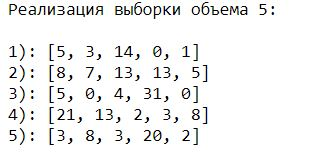
\includegraphics[width=1\linewidth]{vibor_5.jpg}
			\caption{n= 5} %% подпись к рисунку
			\label{ris:experimoriginal} %% метка рисунка для ссылки на него
		\end{minipage}
		\hfill
		\begin{minipage}[h]{0.4\linewidth}
			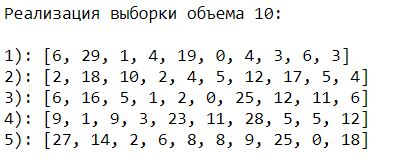
\includegraphics[width=1\linewidth]{vibor_10.jpg}
			\caption{n = 10}
			\label{ris:experimcoded}
		\end{minipage}
	\end{center}
\end{figure}


\text{\large{\textbf {2.1.2 Экспоненциальное распределение}}}\\
\addcontentsline{toc}{section}{2.1.2 Экспоненциальное распределение}
\vspace{5mm}


Используя итоговый из задания 1 для моделирования случайных величин, подчиняющих геометрическому распределению, были построены по 5 реализаций выборок различных объемов(5, 10, 100, 1000, 10**5)
\vspace{5mm}

Вот, пример по  5 реализаций выборки объема 5 и  10 соответственно:

\begin{figure}[h]
	\begin{center}
		\begin{minipage}[h]{0.4\linewidth}
			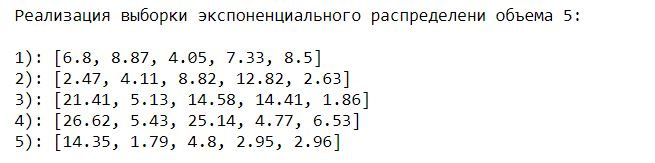
\includegraphics[width=1\linewidth]{vibor_ex_5.jpg}
			\caption{n= 5} %% подпись к рисунку
			\label{ris:experimoriginal} %% метка рисунка для ссылки на него
		\end{minipage}
		\hfill
		\begin{minipage}[h]{0.4\linewidth}
			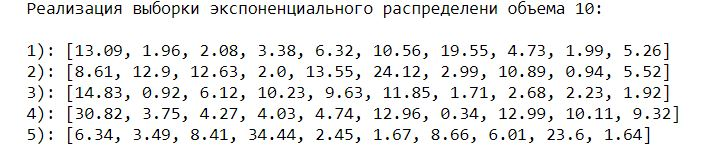
\includegraphics[width=1\linewidth]{vibor_ex_10.jpg}
			\caption{n = 10}
			\label{ris:experimcoded}
		\end{minipage}
	\end{center}
\end{figure}

\newpage
{\large\textit{\textbf{Задание 2.2} Построение эмпирической функции распределения}}
\addcontentsline{toc}{chapter}{Задание 2.2 Построение эмпирической функции распределения}


\vspace{5mm}
	\large{\textbf{Эмпирическая функция распределения}}
\vspace{5mm}

\normalsize{\textbf{Определение 2.}} Для произвольного числа $x \in R$ рассмотрим случайную величину
$$
\mu_n(x) = \sum\limits_{i=1}^n Ind(X_i \leq x )
$$

равную числу элементов выборки меньших или равных $x$. Тогда функция $\hat{F}(x) = \frac{\mu_n (x)}{n} $ называется \textit{эмпирической функцией распределения(э.ф.р)}

\vspace{3mm}
Эмпирическая функция распределения принимает значения $\{0,\frac{1}{n}, \frac{2}{n}, \ldots, \frac{n}{n} \}$

$$
P(\hat{F}(x) = \frac{k}{n}) = C_k^m F^k (x)(1-F(x))^{{n-k}}
$$

\vspace{5mm}
\text{\large{\textbf {2.2.1 Геометрическое распределение}}}\\
\addcontentsline{toc}{section}{2.2.1 Геометрическое распределение}
\vspace{5mm}



Для каждой выборки построим эфр. На каждом графике приведены графики э.ф.р 5 реализаций одинакового объема, а также график функции распределения, помеченный синим цветом.  Для его построения использовался модуль scipy.stats \\
\vspace{5mm}


\begin{figure}[h!]
	\begin{center}
	\begin{minipage}[h]{0.47\linewidth}
		\center{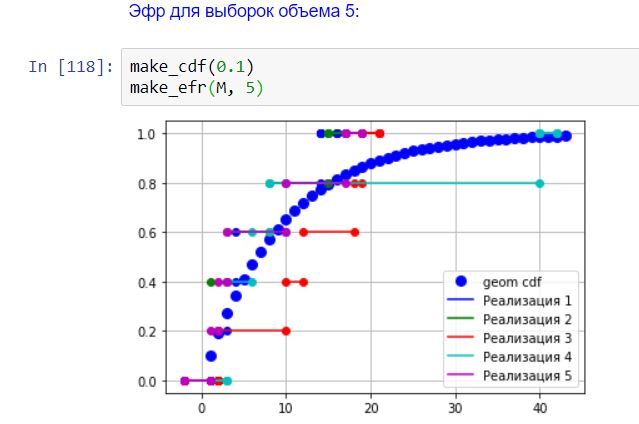
\includegraphics[width=1\linewidth]{efr_5.jpg}} a) \\
	\end{minipage}
	\hfill
	\begin{minipage}[h]{0.47\linewidth}
		\center{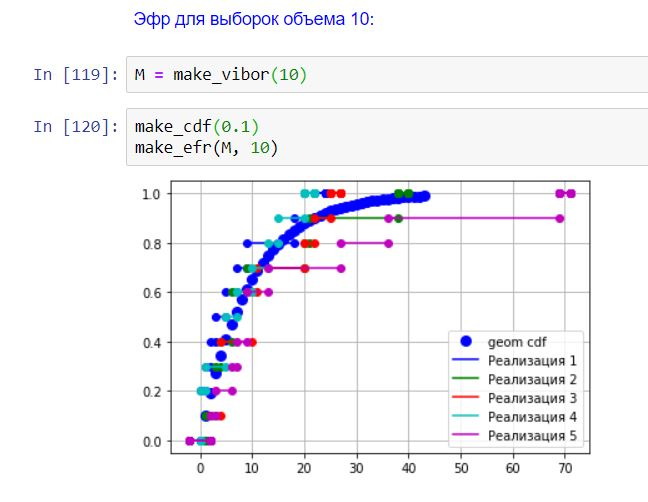
\includegraphics[width=1\linewidth]{efr_10.jpg}} \\b)
	\end{minipage}
	\vfill
	\begin{minipage}[h]{0.47\linewidth}
		\center{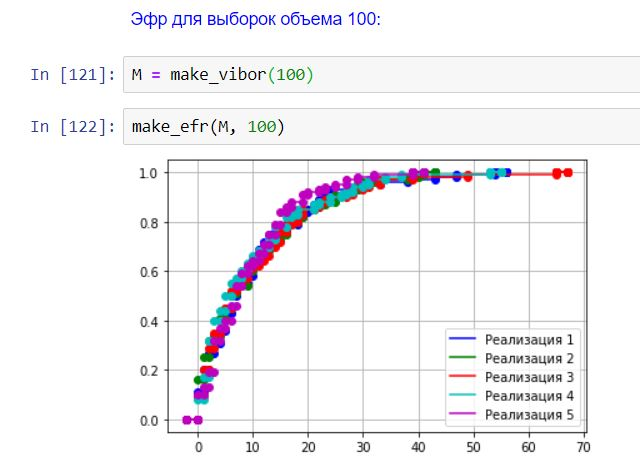
\includegraphics[width=1\linewidth]{efr_100.jpg}} c) \\
	\end{minipage}
	\hfill
	\begin{minipage}[h]{0.47\linewidth}
		\center{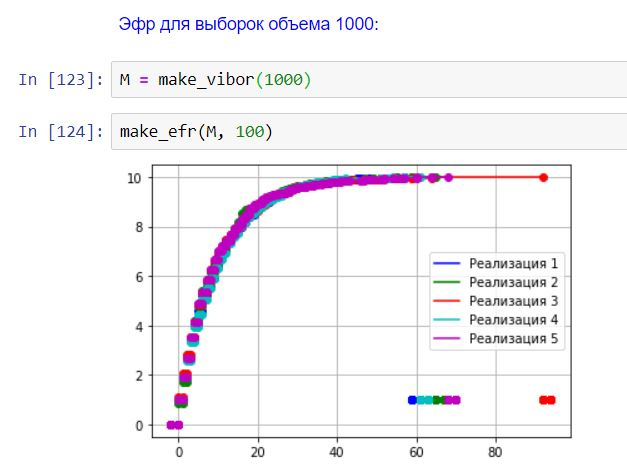
\includegraphics[width=1\linewidth]{efr_1000.jpg}} d) \\
	\end{minipage}
	\hfill
	\begin{minipage}[h]{0.47\linewidth}
		\center{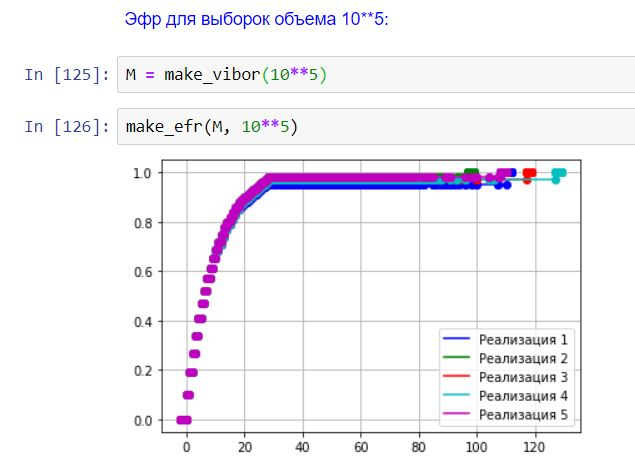
\includegraphics[width=1\linewidth]{efr_103.jpg}} e) \\
	\end{minipage}
	\end{center}
\end{figure}

\newpage
Теперь найдем точную верхнюю границу разности каждой пары эмпирических функций распределения:

Для этого выберет какое-то значение на оси x(например x = 4), и посмотри чему равно $f(x)$ э.ф.р для данного икса.

Приведем результаты для выборок различного объема:
\vspace{5mm}


\begin{figure}[h!]
	\begin{center}
	\begin{minipage}[h]{0.47\linewidth}
		\center{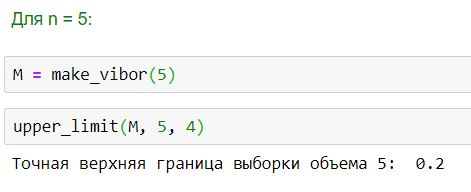
\includegraphics[width=1\linewidth]{up_lim_5.jpg}} n = 5 \\
	\end{minipage}
	\hfill
	\begin{minipage}[h]{0.47\linewidth}
		\center{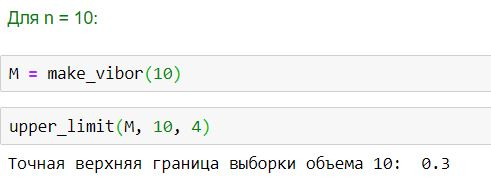
\includegraphics[width=1\linewidth]{up_lim_10.jpg}} n = 10 \\
	\end{minipage}
	\vfill
	\begin{minipage}[h]{0.47\linewidth}
		\center{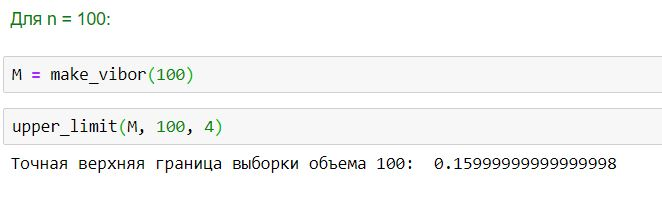
\includegraphics[width=1\linewidth]{up_lim_100.jpg}} n = 100 \\
	\end{minipage}
	\hfill
	\begin{minipage}[h]{0.47\linewidth}
		\center{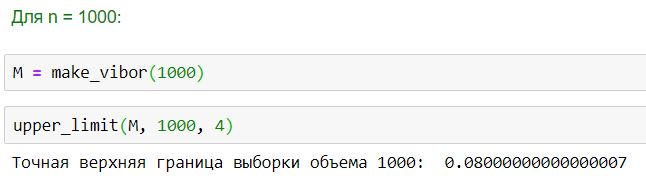
\includegraphics[width=1\linewidth]{up_lim_1000.jpg}} n = 1000  \\
	\end{minipage}
	\hfill
	\begin{minipage}[h]{0.47\linewidth}
		\center{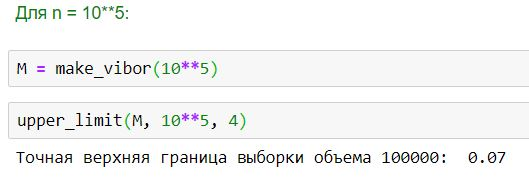
\includegraphics[width=1\linewidth]{up_lim_103.jpg}} n = 100000 \\
	\end{minipage}
	\end{center}
\end{figure}



\newpage
\text{\large{\textbf {2.2.2 Экспоненциальное распределение}}}\\
\addcontentsline{toc}{section}{2.2.2 Экспоненциальное распределение}
\vspace{5mm}

Для каждой выборки построим эфр. На каждом графике приведены графики э.ф.р 5 реализаций одинакового объема, а также график функции распределения, помеченный синим цветом.  Для его построения использовался модуль scipy.stats \\
\vspace{5mm}

\begin{figure}[p]
	\begin{center}
		\begin{minipage}[h!]{0.47\linewidth}
			\center{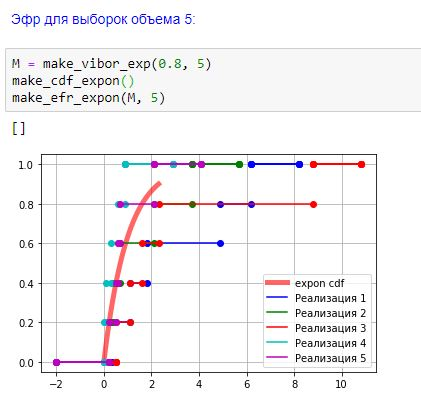
\includegraphics[width=1\linewidth]{efr_exp_5.jpg}} a) \\
		\end{minipage}
		\hfill
		\begin{minipage}[h!]{0.47\linewidth}
			\center{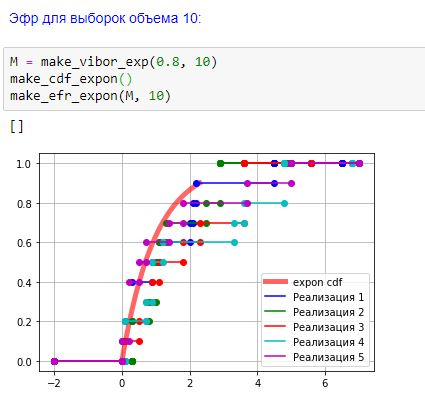
\includegraphics[width=1\linewidth]{efr_exp_10.jpg}} \\b)
		\end{minipage}
		\vfill
		\begin{minipage}[h!]{0.47\linewidth}
			\center{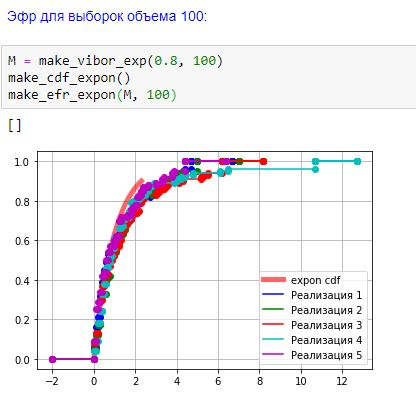
\includegraphics[width=1\linewidth]{efr_exp_100.jpg}} c) \\
		\end{minipage}
		\hfill
		\begin{minipage}[h!]{0.47\linewidth}
			\center{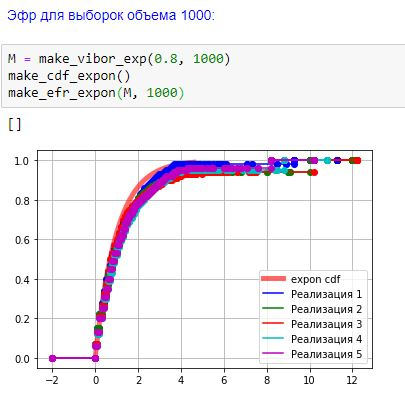
\includegraphics[width=1\linewidth]{efr_exp_1000.jpg}} d) \\
		\end{minipage}
		\hfill
		\begin{minipage}[h!]{0.47\linewidth}
			\center{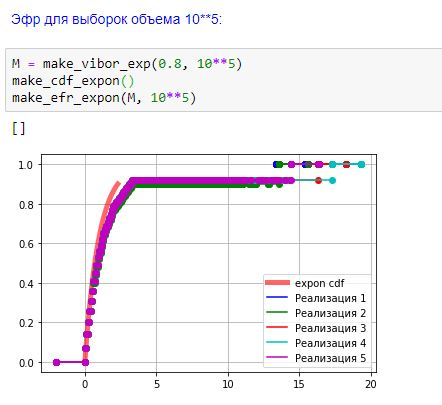
\includegraphics[width=1\linewidth]{efr_exp_103.jpg}} e) \\
		\end{minipage}
	\end{center}
\end{figure}


Теперь найдем точную верхнюю границу разности каждой пары эмпирических функций распределения:

Для этого выберет какое-то значение на оси x(например x = 4), и посмотри чему равно $f(x)$ э.ф.р для данного икса.

Приведем результаты для выборок различного объема:
\vspace{5mm}


\begin{figure}[h!]
	\begin{center}
		\begin{minipage}[h]{0.47\linewidth}
			\center{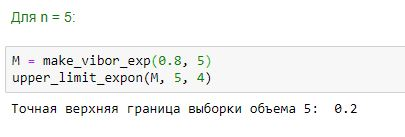
\includegraphics[width=1\linewidth]{up_exp_5.jpg}} n = 5 \\
		\end{minipage}
		\hfill
		\begin{minipage}[h]{0.47\linewidth}
			\center{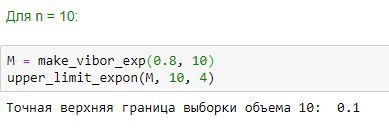
\includegraphics[width=1\linewidth]{up_exp_10.jpg}} n = 10 \\
		\end{minipage}
		\vfill
		\begin{minipage}[h]{0.47\linewidth}
			\center{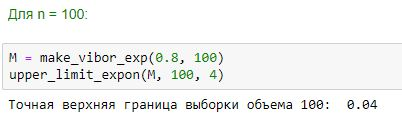
\includegraphics[width=1\linewidth]{up_exp_100.jpg}} n = 100 \\
		\end{minipage}
		\hfill
		\begin{minipage}[h]{0.47\linewidth}
			\center{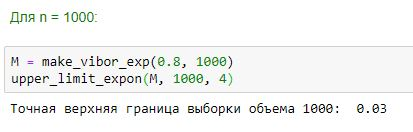
\includegraphics[width=1\linewidth]{up_exp_1000.jpg}} n = 1000  \\
		\end{minipage}
		\hfill
		\begin{minipage}[h]{0.47\linewidth}
			\center{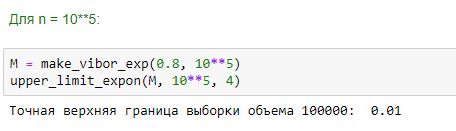
\includegraphics[width=1\linewidth]{up_exp_103.jpg}} n = 100000 \\
		\end{minipage}
	\end{center}
\end{figure}

\newpage
{\large\textit{\textbf{Задание 2.3} Построение вариационного ряда выборки}}
\addcontentsline{toc}{chapter}{Задание 2.3 Построение вариационного ряда выборки}

\vspace{5mm}
\large{\textbf{Вариационный ряд выборки}}
\vspace{5mm}

\normalsize{\textbf{Определение 3.}} Пусть есть 
$$
\vec{X} = (X_1, \ldots , X_n),
$$

где $X_i, i=\overline{1,n} - $независимые одинаково распределенные случайные величины из распределения $\xi$. И $\vec{x} = (x_1, \cdots, x_n)$ является реализацией
имеющейся выборки $\vec{X}$. Отсортируем вектор $\vec{x}$ по возрастанию:
$$
x_{(1)} \leq x_{(2)} \leq \ldots \leq x_{(n)}
$$
Тогда $x_{(1)} = \min(x_1, x_2, \ldots x_n)$, а $x_{(n)} = \max(x_1, x_2, \ldots, x_n)$. Через $X_{(i)}$ 
обозначают случайную величину, которая для каждой реализации выборки
принимает значение $X_{(i)}$. Вектор $(X_{(1)}, X_{(2)}, \ldots, X_{(n)})$ называют вариационным рядом выборки.

\vspace{5mm}
\large{\textbf{Квантиль}}
\vspace{5mm}

\normalsize{\textbf{Определение 4.}} \textit{Квантилью уровня} $\alpha \in (0, 1)$ функции распределения $F(x)$ называется величина $\zeta_\alpha = \sup\{ x: F(x) \leq p \} = F^{-1}(p)$.

\vspace{5mm}
\large{\textbf{Выборочный квантиль}}
\vspace{5mm}

\normalsize{\textbf{Определение 5.}} \textit{Выборочными квантилями } называют квантили выборочного распределения.
\setcounter{secnumdepth}{-1} % убираем нумерацию 
\vspace{5mm}
\section{2.3.1 Геометрическое распределение}
\vspace{5mm}



Для каждой выборки построим вариационный ряд. Вот, примеры вариационных рядов для выборок объема n = 5 и для n = 10:

\begin{figure}[h!]
	\begin{center}
		\begin{minipage}[h]{0.4\linewidth}
			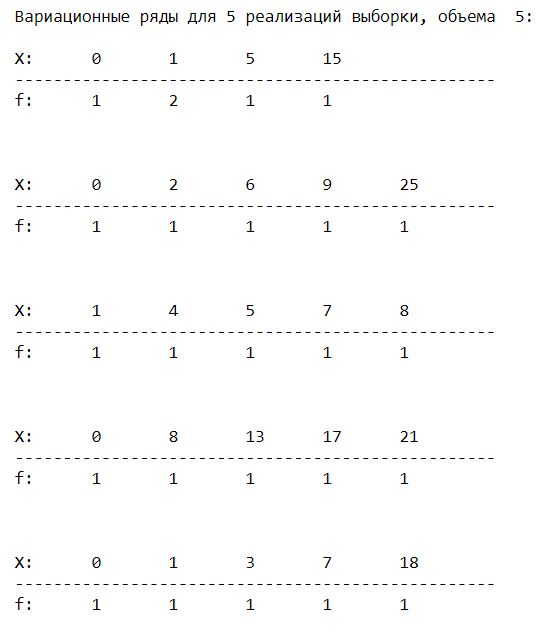
\includegraphics[width=1\linewidth]{var_ser_5.jpg}
			\caption{n = 5} %% подпись к рисунку
		\end{minipage}
		\hfill
		\begin{minipage}[h]{0.4\linewidth}
			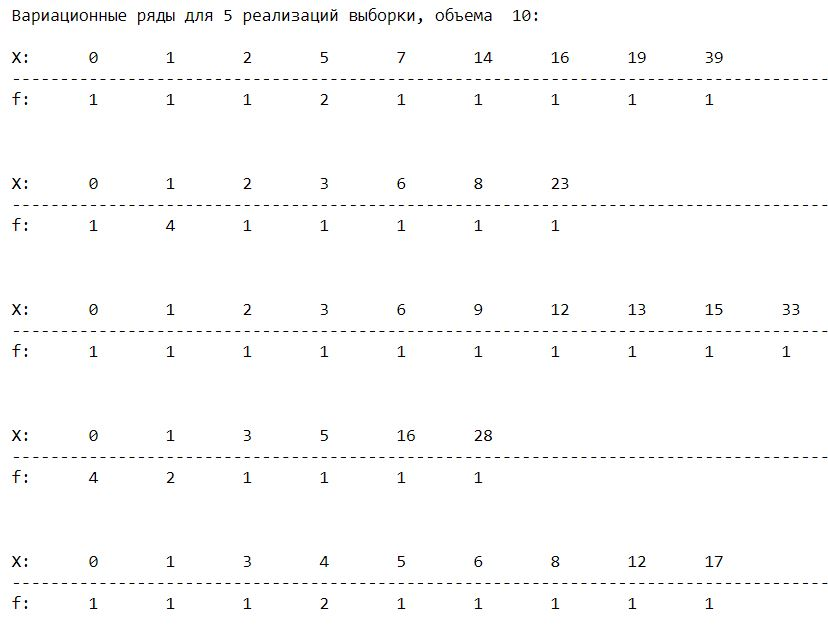
\includegraphics[width=1\linewidth]{var_ser_10.jpg}	
			\caption{n = 10} %% подпись к рисунку
		\end{minipage}

	\end{center}
\end{figure}


\vspace{5mm}



\newpage

	Перейдем к нахождению выборочной квантили.
	
	Поясним простыми словами на примере уровня квантиля  0.1, что такое выборочная квантиль:
	
	\vspace{3mm}
	Выборочная квантиль уровня 0,1 - это точка, левее которой (включая её саму) лежит не менее 10\% всей выборки, и правее которой (снова включая её саму) - не менее $100\%-10\%=90\%$ выборки.
	\vspace{5mm}
	
	 Будем искать выборочную квантиль графическим способом: проведем прямую $y =$(уровень квантиля) до пересечения с графиком. И определим  $x$, при котором прямая пересекает график. Если точка пересечения одна, то именно это значения $x$ и будет выборочной квантиль. А если пересечение проходит по отрезку, то квантилей будет много. Например, если отрезок от 3 до 4 является прямой $y$, то квантилью будет любое число от 3 до 4. ля определённости в практической статистике в таких случаях выбирают по какому-то правилу одно из чисел "отрезка квантилей". Например, середину отрезка - в данном случае 3,5.
	 
	 Ниже показано в первой строчке расчет выборочной квантильи уровня 0.1, 0.5, 0.7, а затем графическое предстваление для геометрического распределения. Жирной, серой чертой как раз и проведена линия уровня, по которой мы находим квантиль
	 
\begin{figure}[h!]
	\begin{center}
		\begin{minipage}[h]{0.47\linewidth}
			\center{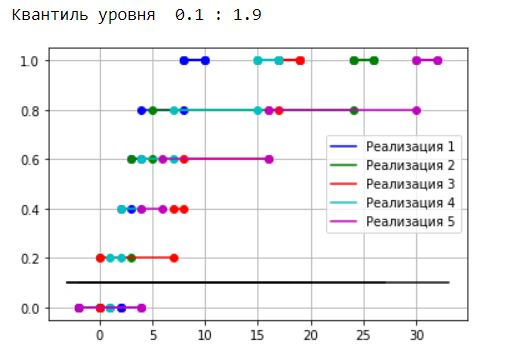
\includegraphics[width=1\linewidth]{quantile01.jpg}} a = 0.1 \\
		\end{minipage}
		\hfill
		\begin{minipage}[h]{0.47\linewidth}
			\center{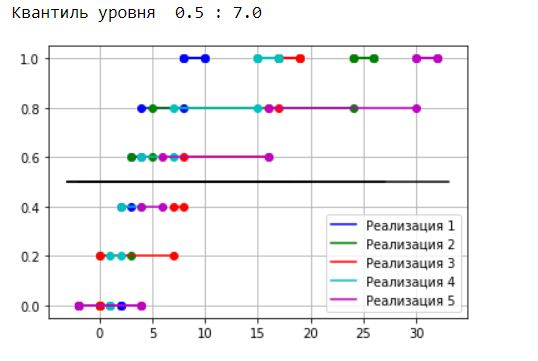
\includegraphics[width=1\linewidth]{quantile05.jpg}} a = 0.5 \\
		\end{minipage}
		\vfill
		\begin{minipage}[h]{0.47\linewidth}
			\center{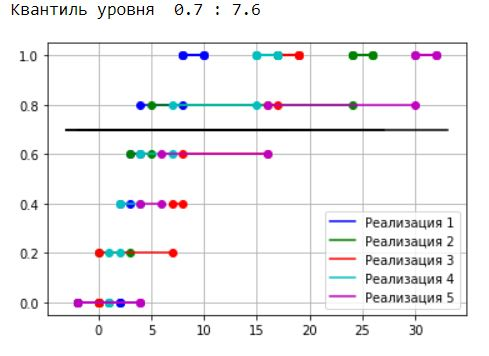
\includegraphics[width=1\linewidth]{quantile07.jpg}} a = 0.7 \\
		\end{minipage}
	\end{center}
\end{figure}

\newpage
\vspace{5mm}
\text{\large{\textbf {2.3.2 Экспоненциальное распределение}}}\\
\addcontentsline{toc}{section}{2.3.2 Экспоненциальное распределение}
\vspace{5mm}



Для каждой выборки построим вариационный ряд. Вот, примеры вариационных рядов для выборок объема n = 5 и для n = 10:

\begin{figure}[h!]
	\begin{center}
		\begin{minipage}[h]{0.4\linewidth}
			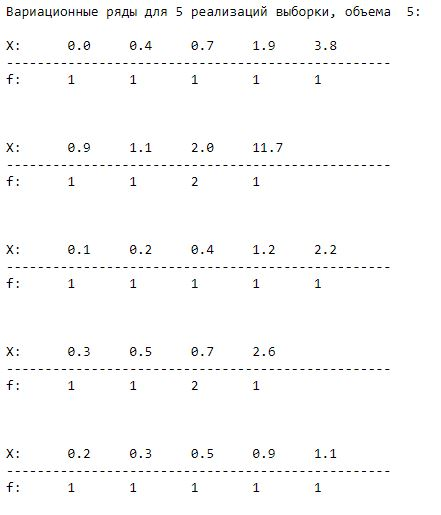
\includegraphics[width=1\linewidth]{var_ser_exp_5.jpg}
			\caption{n = 5} %% подпись к рисунку
		\end{minipage}
		\hfill	
		\begin{minipage}[h]{0.4\linewidth}
			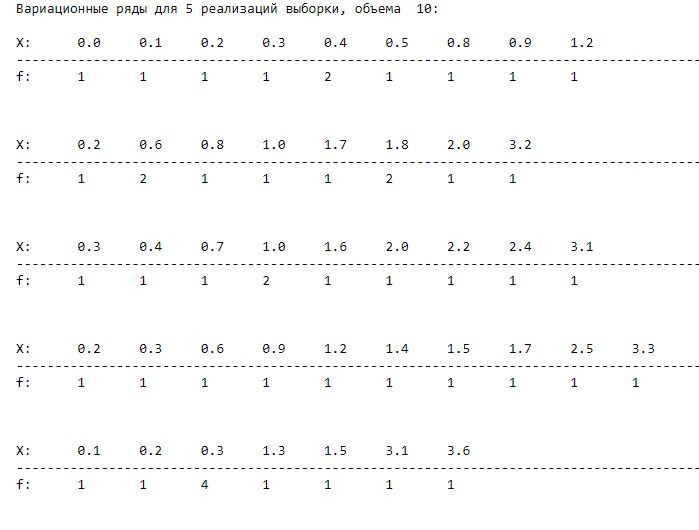
\includegraphics[width=1\linewidth]{var_ser_exp_10.jpg}	
			\caption{n = 10} %% подпись к рисунку/
		\end{minipage}
		
	\end{center}
\end{figure}


\newpage
{\large\textit{\textbf{Задание 2.4} Построение гистограммы и полигон частот}}
\addcontentsline{toc}{chapter}{Задание 2.4 Построение гистограммы и полигон частот}

\vspace{5mm}
\large{\textbf{Гистограмма}}
\vspace{5mm}

\normalsize{\textbf{Определение 4.}}Для непрерывной случайной величины $\xi$, обладающей непрерывной плотностью $f(x)$, также можно построить по соответствующей выборке $X = (X_1, \ldots, X_n)$ статистический аналог $\hat{f_n} (x)$ для плотности $f(x)$, который называется \textit{гистограммой}  

\vspace{5mm}
\large{\textbf{Полигон частот}}
\vspace{5mm}

\normalsize{\textbf{Определение 5.}} Наряду с гистограммой, в качестве приближения для неизвестной теоретической плотности $ f(x)$ можно использовать кусочно-линейный график, называемый \textit{полигоном частот}, и который строится так: если построена гистограмма $\hat{f_n} (x)$, то ординаты, соответствующие серединам интервалов группировки, последовательно соединяют отрезками прямых. 

\vspace{5mm}
\text{\large{\textbf {2.4.1 Геометрическое распределение}}}\\
\addcontentsline{toc}{section}{2.4.1 Геометрическое распределение}
\vspace{5mm}


Ниже представлены гистограммы частот для геометрического распределения:\\

\begin{figure}[h!]
	\begin{center}
		\begin{minipage}[h]{0.47\linewidth}
			\center{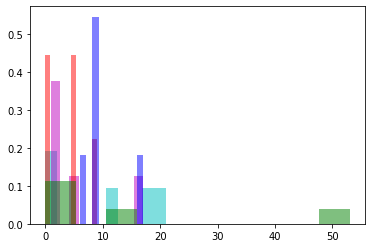
\includegraphics[width=1\linewidth]{fotos/Geom/Gist/g5.png}} a) \\
		\end{minipage}
		\hfill
		\begin{minipage}[h]{0.47\linewidth}
			\center{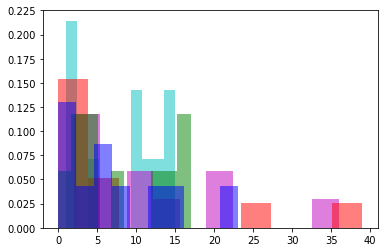
\includegraphics[width=1\linewidth]{fotos/Geom/Gist/g10.png}} \\b)
		\end{minipage}
		\vfill
		\begin{minipage}[h]{0.47\linewidth}
			\center{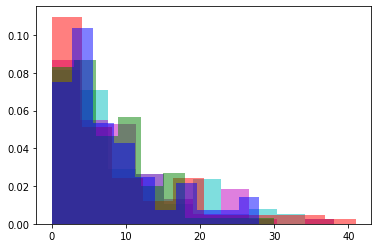
\includegraphics[width=1\linewidth]{fotos/Geom/Gist/g100.png}} c) \\
		\end{minipage}
		\hfill
		\begin{minipage}[h]{0.47\linewidth}
			\center{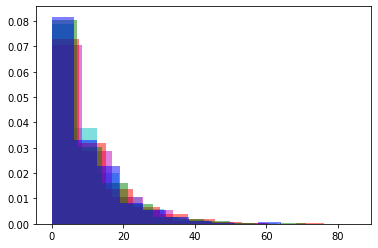
\includegraphics[width=1\linewidth]{fotos/Geom/Gist/g1000.png}} d) \\
		\end{minipage}
		\hfill
		\begin{minipage}[h]{0.47\linewidth}
			\center{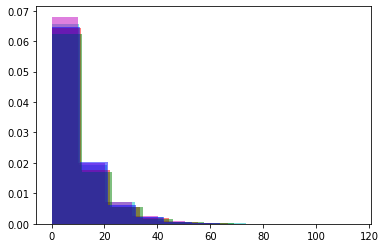
\includegraphics[width=1\linewidth]{fotos/Geom/Gist/g103.png}} e) \\
			\vspace{10mm}
		\end{minipage}
	\end{center}
\end{figure}

Ниже представлены полигоны частот для геометрического распределения:\\
\begin{figure}[h!]
	\begin{center}
		\begin{minipage}[h!]{0.47\linewidth}
			\center{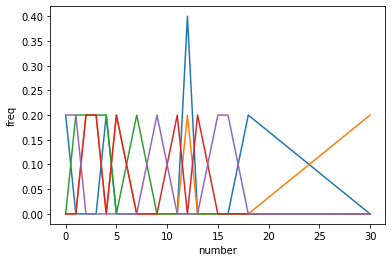
\includegraphics[width=1\linewidth]{fotos/Geom/Polig/pol5.png}} a) \\
		\end{minipage}
		\hfill
		\begin{minipage}[h!]{0.47\linewidth}
			\center{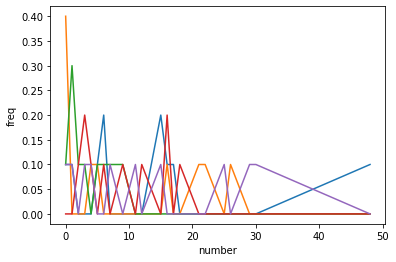
\includegraphics[width=1\linewidth]{fotos/Geom/Polig/pol10.png}} \\b)
		\end{minipage}
		\vfill
		\begin{minipage}[h!]{0.47\linewidth}
			\center{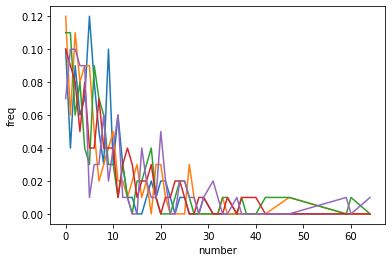
\includegraphics[width=1\linewidth]{fotos/Geom/Polig/pol100.png}} c) \\
		\end{minipage}
		\hfill
		\begin{minipage}[h!]{0.47\linewidth}
			\center{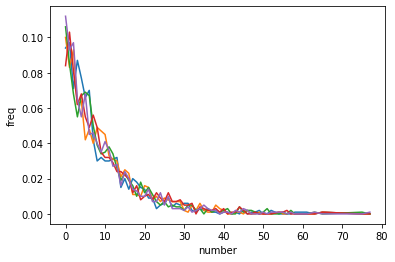
\includegraphics[width=1\linewidth]{fotos/Geom/Polig/pol1000.png}} d) \\
		\end{minipage}
		\hfill
		\begin{minipage}[h]{0.47\linewidth}
			\center{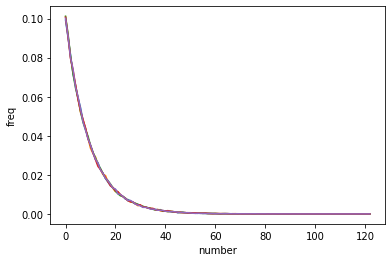
\includegraphics[width=1\linewidth]{fotos/Geom/Polig/pol103.png}} e) \\
		\end{minipage}
	\end{center}
\end{figure}

\newpage
$$
$$

\newpage
$$
$$

\newpage
$$
$$

\text{\large{\textbf {2.4.2 Экспоненциальное распределение}}}\\
\addcontentsline{toc}{section}{2.4.2 Экспоненциальное распределение}

Ниже представлены гистограммы частот для экспоненциального  распределения:\\

\begin{figure}[h!]
	\begin{center}
		\begin{minipage}[h]{0.47\linewidth}
			\center{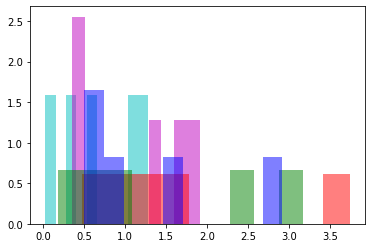
\includegraphics[width=1\linewidth]{fotos/Expon/Gist/g5.png}} a) \\
		\end{minipage}
		\hfill
		\begin{minipage}[h]{0.47\linewidth}
			\center{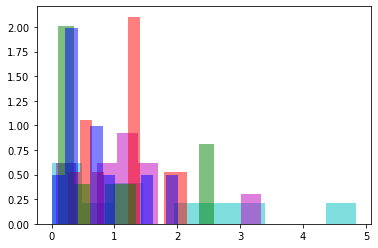
\includegraphics[width=1\linewidth]{fotos/Expon/Gist/g10.png}} \\b)
		\end{minipage}
		\vfill
		\begin{minipage}[h]{0.47\linewidth}
			\center{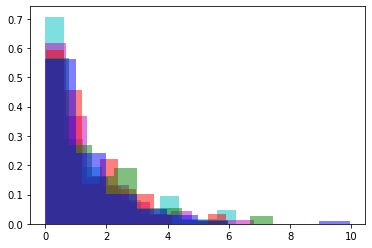
\includegraphics[width=1\linewidth]{fotos/Expon/Gist/g100.png}} c) \\
		\end{minipage}
		\hfill
		\begin{minipage}[h]{0.47\linewidth}
			\center{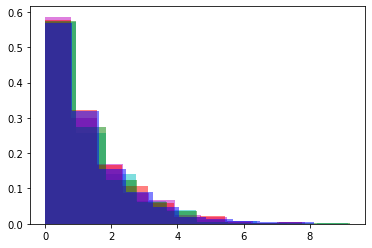
\includegraphics[width=1\linewidth]{fotos/Expon/Gist/g1000.png}} d) \\
		\end{minipage}
		\hfill
		\begin{minipage}[h]{0.47\linewidth}
			\center{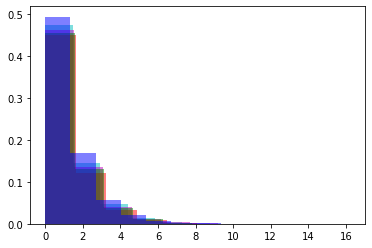
\includegraphics[width=1\linewidth]{fotos/Expon/Gist/g103.png}} e) \\
			\vspace{10mm}
		\end{minipage}
	\end{center}
\end{figure}

\newpage
Ниже представлены полигоны частот для экспоненциального  распределения:\\

\begin{figure}[h!]
	\begin{center}
		\begin{minipage}[h]{0.47\linewidth}
			\center{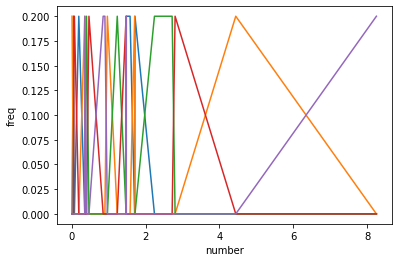
\includegraphics[width=1\linewidth]{fotos/Expon/Poligon/pol5.png}} a) \\
		\end{minipage}
		\hfill
		\begin{minipage}[h]{0.47\linewidth}
			\center{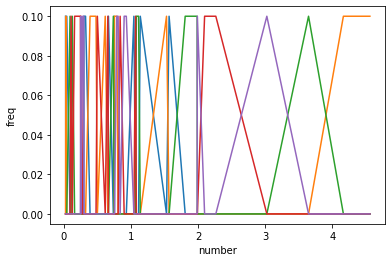
\includegraphics[width=1\linewidth]{fotos/Expon/Poligon/pol10.png}} \\b)
		\end{minipage}
		\vfill
		\begin{minipage}[h]{0.47\linewidth}
			\center{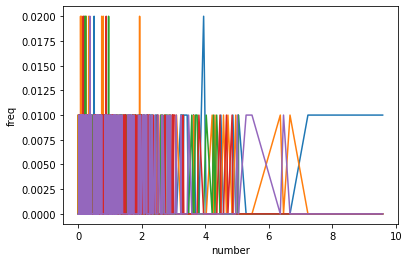
\includegraphics[width=1\linewidth]{fotos/Expon/Poligon/pol100.png}} c) \\
		\end{minipage}
		\hfill
		\begin{minipage}[h]{0.47\linewidth}
			\center{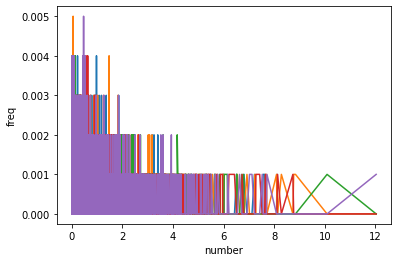
\includegraphics[width=1\linewidth]{fotos/Expon/Poligon/pol1000.png}} d) \\
		\end{minipage}
		\hfill
		\begin{minipage}[h]{0.47\linewidth}
			\center{\includegraphics[width=1\linewidth]{fotos/Expon/Poligon/pol103.png}} e) \\
			\vspace{50mm}
		\end{minipage}
	\end{center}
\end{figure}


\begin{thebibliography}{99}
	\bibitem{rt1} 
	\bibitem{rt2} \href{https://towardsdatascience.com/what-is-exponential-distribution-7bdd08590e2a}{ссылка1}
	\bibitem{rt3}  \href{https://www.statisticshowto.datasciencecentral.com/exponential-distribution/}{ссылка2}
	\bibitem{rt4}  // \href{http://www.ams.jhu.edu/~dan/550.435/notes/COURSENOTES435.pdf}{ссылка3}
	\bibitem{rt5}  // \href{http://www.obzh.ru/nad/4-3.html}{ссылка4}
\end{thebibliography}

\end{document}